% \documentclass[tikz, border=10pt]{standalone}

\definecolor{sv}{HTML}{90F7EC}
\definecolor{m1}{HTML}{FDEB71}
\definecolor{m2}{HTML}{FEB692}
\definecolor{ge}{HTML}{ABDCFF}

\usetikzlibrary{
  decorations.pathreplacing,    % paths with shoapes of curly braces
  positioning,     % positions like above of node
  fit              % legend bounding box fitting all nodes
}
\tikzset{
    node distance=4ex and 4ex,
    % on grid,  % node distance from the centers
    every node/.style = {
        rectangle,
        minimum width=5em,
        minimum height=3ex,
        text depth=1pt,
        draw,
        outer sep = 2pt,
        inner sep = 3pt
    },
    every edge/.style = {->,draw},
    virtual/.append style = {draw=none, circle, minimum width=1em},
    % virtual/.append style = {draw, color=black!50},   % debugging purposes
    several/.append style = {fill = sv},
    m1/.append style = {fill = m1},
    m2/.append style = {fill = m2},
    gxe/.append style = {fill = ge},
    aux/.append style = {fill = none},
    legendkey/.append style = {minimum width=3ex},
    legendtext/.append style = {draw=none, fill = black!10},
    ->,        % arrows for all
    >=stealth  % arrow type
}
\pgfdeclarelayer{background}
\pgfsetlayers{background,main}

% \begin{document}

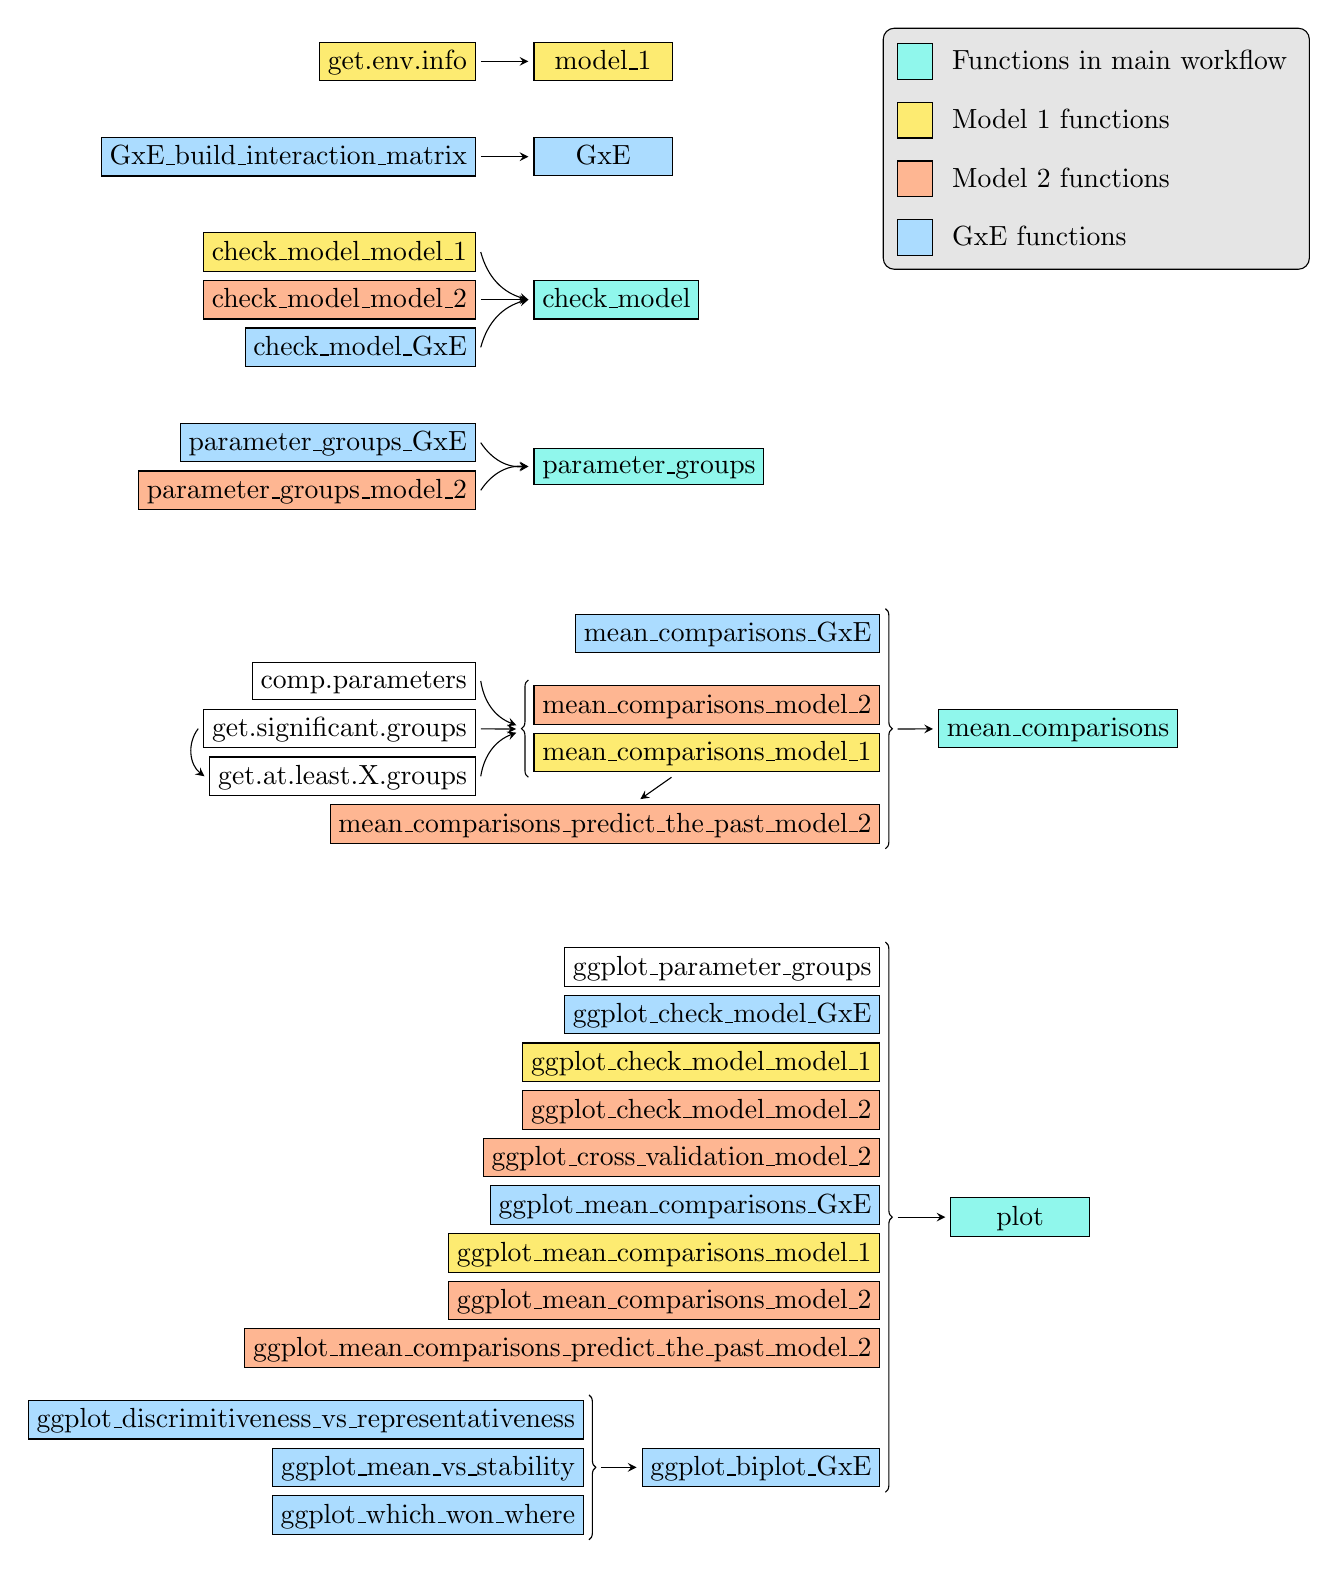
\begin{tikzpicture}

  %% Model 1
  \node [m1] (GEI) {get.env.info};
  \node [m1, right=of GEI] (m1) {model\_1};
  \draw (GEI) to (m1);
  
  
  %% GxE
  \node [gxe, below=of GEI.east, left, yshift=-4ex] (GEBIM) {GxE\_build\_interaction\_matrix};
  \node [gxe, right=of GEBIM] (GxE) {GxE};
  \draw (GEBIM) to (GxE);


  %% check_model
  \node [m1, below=of GEBIM.east, left, yshift=-4ex] (cmm1) {check\_model\_model\_1};
  \node [m2, below=of cmm1.east, left] (cmm2) {check\_model\_model\_2};
  \node [gxe, below=of cmm2.east, left] (cmgxe) {check\_model\_GxE};
  
  \node [several, right=of cmm2] (cm) {check\_model};
  
  \draw [bend right] (cmm1.east) to (cm.west);
  \draw (cmm2) to (cm);
  \draw [bend left] (cmgxe.east) to (cm.west);


  %% parameter_groups
  \node [gxe, below=of cmgxe.east, left, yshift=-4ex] (pggxe) {parameter\_groups\_GxE};
  \node [m2, below=of pggxe.east, left] (pgm2) {parameter\_groups\_model\_2};

  \node [several, right=of pgm2, yshift=2ex] (pg) {parameter\_groups};

  \draw [bend right] (pggxe.east) to (pg.west);
  \draw [bend left] (pgm2.east) to (pg.west);


  %% mean_comparisons
  \node [aux, below=of pgm2.east, left, yshift=-12ex] (cp) {comp.parameters};
  \node [aux, below=of cp.east, left] (gsg) {get.significant.groups};
  \node [aux, below=of gsg.east, left] (galXg) {get.at.least.X.groups};
  
  \node [m1, right=of galXg, yshift=2ex] (MCM1) {mean\_comparisons\_model\_1};
  \node [m2, above=of MCM1.east, left] (MCM2) {mean\_comparisons\_model\_2};
  \node [gxe, above=of MCM2.east, left, yshift=2ex] (MCGxE) {mean\_comparisons\_GxE};
  \node [m2, below=of MCM1.east, left, yshift=-2ex] (MCPPM2) {mean\_comparisons\_predict\_the\_past\_model\_2};
  
  \node [virtual, above=of MCM1.west, yshift=-4ex, xshift=4pt] (X1) {};
  \node [virtual, above=of MCM1.east, yshift=-4ex, xshift=-4pt] (X2) {};
  
  \node [several, right=of MCM1, yshift=2ex] (MC) {mean\_comparisons};
  
  \draw [bend right=45] (gsg.west) to (galXg.west);
  \draw (MCM1) to (MCPPM2);
  
  % braces
  \draw [-, decorate,decoration=brace] (MCM1.south west) -- (MCM2.north west);
  \draw [-, decorate,decoration=brace] (MCGxE.north east) -- (MCPPM2.south east);
  
  \draw [bend right] (cp.east) to (X1);
  \draw (gsg) to (X1);
  \draw [bend left] (galXg.east) to (X1);
  \draw (X2) to (MC);
 

  %% plot
  \node [aux, below=of MCPPM2.east, left, yshift=-8ex] (GPG) {ggplot\_parameter\_groups};
  \node [gxe, below=of GPG.east, left] (GCMGxE) {ggplot\_check\_model\_GxE};
  \node [m1, below=of GCMGxE.east, left] (GCMM1) {ggplot\_check\_model\_model\_1};
  \node [m2, below=of GCMM1.east, left] (GCMM2) {ggplot\_check\_model\_model\_2};
  \node [m2, below=of GCMM2.east, left] (GCVM2) {ggplot\_cross\_validation\_model\_2};
  \node [gxe, below=of GCVM2.east, left] (GMCGxE) {ggplot\_mean\_comparisons\_GxE};
  \node [m1, below=of GMCGxE.east, left] (GMCM1) {ggplot\_mean\_comparisons\_model\_1};
  \node [m2, below=of GMCM1.east, left] (GMCM2) {ggplot\_mean\_comparisons\_model\_2};
  \node [m2, below=of GMCM2.east, left] (GMCPPM2) {ggplot\_mean\_comparisons\_predict\_the\_past\_model\_2};
  
  \node [gxe, below=of GMCPPM2.east, left, yshift=-6ex] (GBGxE) {ggplot\_biplot\_GxE};
  \node [gxe, left=of GBGxE] (GMS) {ggplot\_mean\_vs\_stability};
  \node [gxe, above=of GMS.east, left] (GDR) {ggplot\_discrimitiveness\_vs\_representativeness};
  \node [gxe, below=of GMS.east, left] (GWWW) {ggplot\_which\_won\_where};

  \draw [-, decorate,decoration=brace] (GDR.north east) -- (GWWW.south east)
    node [midway, virtual, xshift=-4pt] (X3) {};
    
  \draw [-, decorate,decoration=brace] (GPG.north east) -- (GBGxE.south east)
    node [midway, virtual, xshift=-4pt] (X4) {};
  
  \node [several, right=of X4] (P) {plot};
  
  \draw (X3) to (GBGxE);
  \draw (X4) to (P);

  %% legend
  \node[several,legendkey]  (LS)  [right=of m1, xshift=6em] {};
  \node[right,legendtext] (LStext) at (LS.east) {Functions in main workflow};

  \node[m1,legendkey]  (LM1)  [below=of LS,yshift=3ex] {};
  \node[right,legendtext] at (LM1.east) {Model 1 functions};

  \node[m2,legendkey]  (LM2)  [below=of LM1,yshift=3ex] {};
  \node[right,legendtext] at (LM2.east) {Model 2 functions};

  \node[gxe,legendkey]  (LGxE)  [below=of LM2,yshift=3ex] {};
  \node[right,legendtext] at (LGxE.east) {GxE functions};

  %% legend bounding box
  \begin{pgfonlayer}{background}
    \node[
      fill=black!10,
      rounded corners,
      fit = (LS) (LGxE) (LStext)
    ] {};
  \end{pgfonlayer}


\end{tikzpicture}

% \end{document}